\documentclass[12pt]{report}

\usepackage{setspace}
%\setstretch{2.5} % for custom spacing
\setlength{\parindent}{4em}

\usepackage{fancyvrb}
\usepackage{graphicx}
\usepackage{geometry}

\geometry{letterpaper, portrait, margin=1in}

%%%Title Page%%%
\title{
   
\includegraphics[scale=.45]{uga.PNG}\\
   Lab 06
   \bigbreak Designing and Building a Digital Tachometer\\...\\
   Zachary Davis
}

\author{
{\normalsize
\begin{tabular}{l r}
\textbf{Thomas Kruegler} & \textbf{Zachary Davis}\\
tkruegler@uga.edu & zachdav@uga.edu\\
\hline
Lab Part 1 & Software Development\\
Lab Part 2 & Testing w/ Function Generator\\
Lab Part 3 & Calibrating/Smoothing Measurements\\
\end{tabular}
}
}

\date{\bigskip
\today}
%%%%%%%%%%%%


\begin{document}
\maketitle
\section*{Introduction}
	\paragraph*{}
		This project presents a way to create a digital tachometer on the EVB Board.  Due to timing constraints on the semester we were unable to actually connect the motor to the input pins on the EVB Board.  As a replacement we used a function generator and design a program that will echo out the frequency to the terminal which is equal to the RPM.  This means that this lab, which was intented to be a lot like the last no longer had a hardware component.
   \paragraph*{}
      This project was entirely about the construction of software that focused on the concepts of interrupts.  The intention of the program was to interrupt at 2 sequential rising edges from the function generator or a motor and calculate the rotations per minute.  The core design of the program is determining how many clock eges occur between the two rising edges and relate that with the known frequency of the HC11 CPU to determine the RPM of the motor or frequency of the function.
\section*{Lab Procedure}
	\paragraph*{}
		The beginning of the project focused on the very small main routine.  The focus of the main is to focus on the interrupt.  That is exactly what the main does it waits for one edge capture it then waits for the second and does the same.  To do this however you cannot just wait.  You first need to decide which of the three input capture available you want to use.  Once we determined to use Input Capture 1 we needed to define three registers.  We need to set the one bit of the T Flag address corresponding to IC1 to 1.  We also had to do the same with the T Mask.  The defference between the two however is that we need to reset the T Flag bit back to one after every interrupt.  The last thing that needs to be set is what will cause an interrupt to be triggered.  To select a rising edge we set the IC1 edge bit 1 and 2 to 01.  Now the initialization of the Input capture is ready.  Have the anode of the function generator go into PA2 and the cathode to go to ground.
	\paragraph*{}
		At this point we have an EVB board connect to a function generator which is initialized and ready to wait for an interrupt on rising edges.  We now needed to define what the program was to do when an interrupt is actually triggered.  To do that we need to understand what an interrupt does.  When the CPU gets interrupted by the Input Capture 1 it looks at its predetermined vector and goes to the address that is stored there.  However on the EVB Board those vectors are all in EPROM.  To solve this the developers defined sudo vectors.  So when the CPU gets interrupted it looks at the correlated vector for an address which directs it to the address of a predetermined sudo-vector.  Those locations are all listed and 3-bytes wide.  That is the perfect amount of space to store jump to an address at that location.  It has to be that way because the CPU believes that it is already running the interrupt subroutine so you cannot just give it an address you need to give it an instruction.
	\paragraph*{}
		Now you have defined a subroutine called CAPTURE and within the program defined what is to occur when an interrupt happens that is the main focus of the lab.  The rest of the lab is just a combination of everything we have learned in the previous labs to compute the RPM with the information we have and echo it back to the terminal.  To do this we did need to understand the Timer Input Capture or TIC.  The TIC is a running counter that increments on every clock cycle of the HC11 CPU and wraps around on an overflow.  This means that as the first rising edge occurs and the CPU interrupts to capture we store the TIC in a variable.  We then used a variable to toggle between 0 and 1 to tell the program whether this was the first or second interrupt in the measurement.
	\paragraph*{}
		With this information we are able to write a subroutine to find the difference between these two values and that will tell us how many clock cycles occured between the two interrupts, which directly correlate with the clock cycles between rising edges in the function.  There are however two situations.  In one case both interrupt happen before a wrap and the difference is just T2-T1.  However there is a second case where a wrap occurs between interrupts.  When this happens we needed to subtract T1 from Max and add T2.  What that is doing is esentially the same as the first equation by removing the added difference caused by the wrap.  To determine which of these cases is occuring is as simple as determing which is larger T1 or T2.  If T2 is bigger it is case one and if it is smaller it is case two.
	\paragraph*{}
		We now have a value equal to the number of clock cylces that occured between rising edges.  Another way to say that is the number of clock cycles that occur in one period or one rotation of the motor or function.  All we need to do now is relate that value to that of the clock of the HC11 CPU.  To do that is simply the clock divided by the pulse.  However the clock of the HC11 is 2 MHz which is to large for assmebly.  To do the division we first divided both the numerator and denominator by 31 so that both are garunteed to fit in 2-bytes.  While in theory this produces an exactly equal ratio because assmebly truncates decimal places this is what causes the error on the final results.  That all being said we have effectively found the RPM of the motor or frequency of the function.
\section*{Conclusion}
	\paragraph*{}
		This lab at first seemed like a vary large undertaking, but that is only because of how large the program was compared to anything we have done before.  The idea of interrupts was foriegn to us before this and writing softare that is dictated by the CPU rather than dictating is different.  That being said, it opens up many new possiblies of what you can do as a program, one being this tachometer.  There were somthings that i did not get to in the summary.  First of all we did not take on measurement, we took thirty and averaged the results to attempt to retrieve a more accurate result.  While this helped we also made a smoothing routine that truncated the least significant digits.  While we know that this costs a loss of percision it is the percision that that gave that led to inaccuracy.  If there was anyhing I could improve on in this lab it would be that.  It would be to difficult to implement a correcting equation because of the lack of decimals and tendancy to cause overflow.  All things considered this lab taught me and my partner the concept of interupts and after this lab I feel fairly confident in my ability to complete any project in assembly with microcontrollers.

\section*{References}
	\paragraph*{}
		N/A

\section*{Appendix A: Hardware Schematic}
	\begin{center}
	  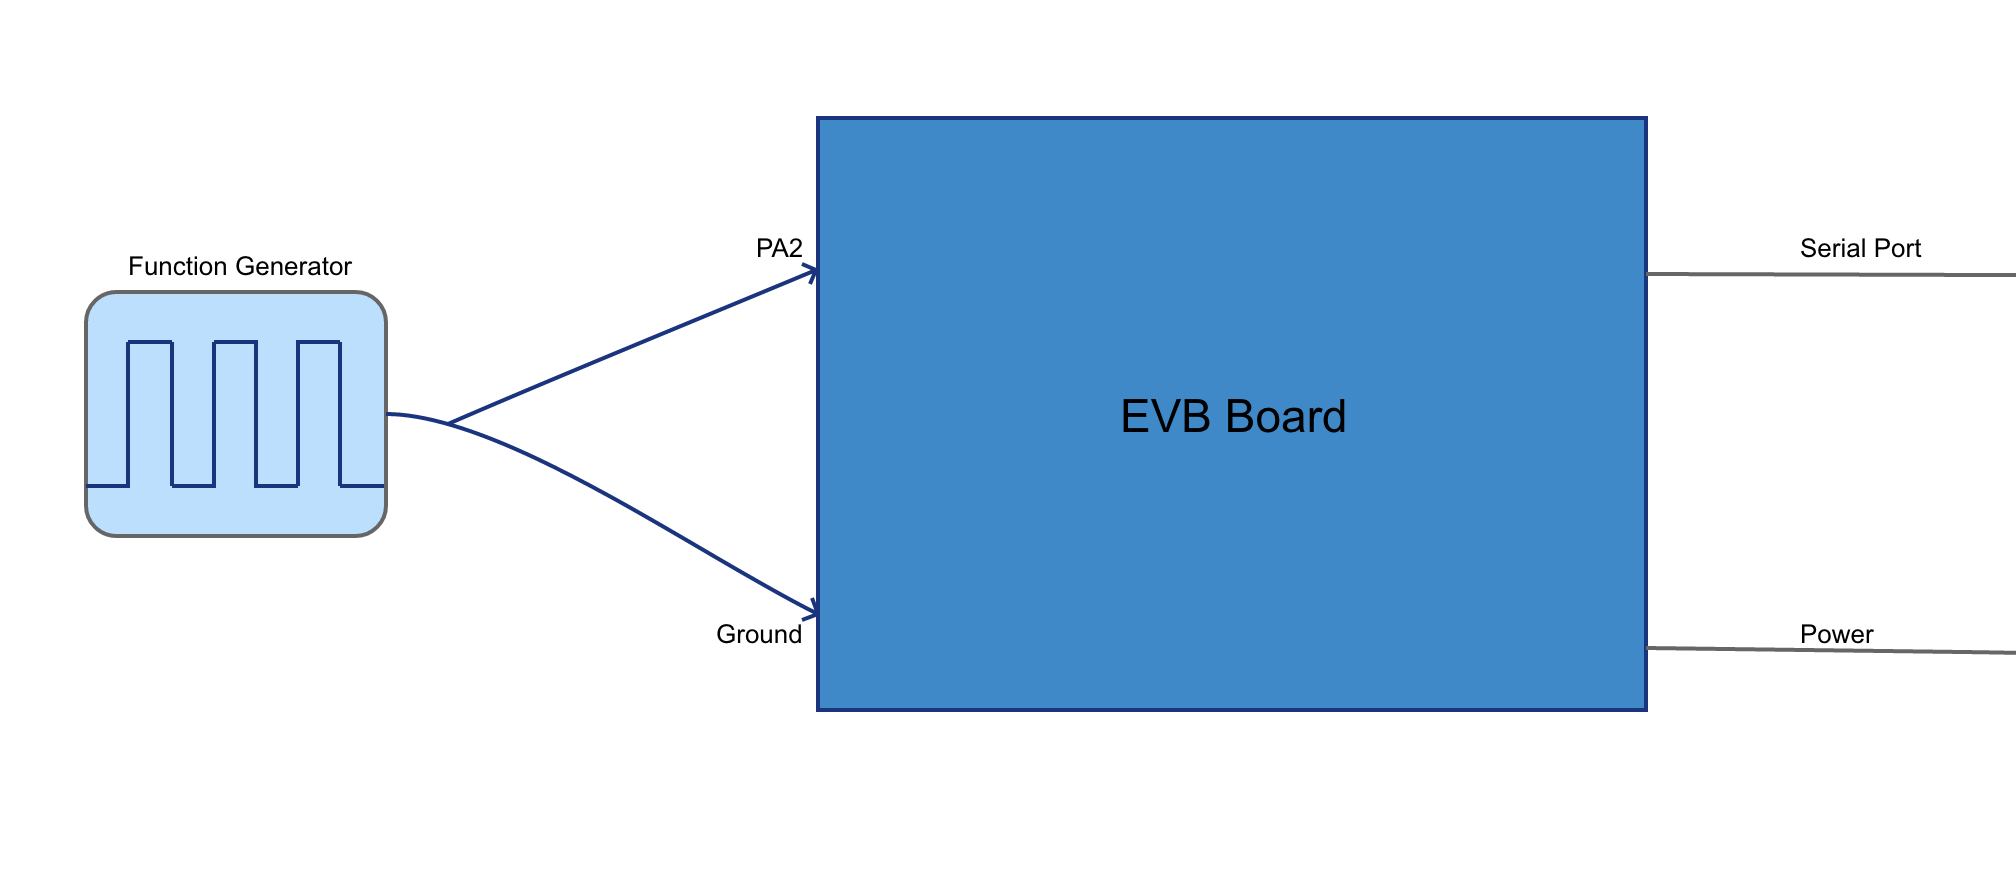
\includegraphics[scale=.45]{HS.PNG}\\
	\end{center}

\section*{Appendix B: Pseudo Code For The Software Developed}
	\begin{Verbatim}[frame=single, fontsize=\footnotesize]
****************************************************************************************
Define all of the constants needed for the entirity of the whole program.
Define the values of the three Input Capture Registers.
Define the addresses of all the registers and results need for the program.
Define the address of the Binary to Binary Coded Decimal addresses.
Define the address of the BUFFALO utility subroutines.
****************************************************************************************

****************************************************************************************
Define the output prompt and units to print at the end of the program.
Create error messages to be used for debugging if the program goes wrong.
****************************************************************************************

****************************************************************************************
Make sure the BUFFALO sudo-vector will direct to program to CAPTURE.
****************************************************************************************

****************************************************************************************
Define the loaction of all the variables needed for the program.
Instantiate space for both TIC interrupt grabs.
Instantiate a counter to stop after X measurements.
Instantiate a toggle to switch between storing T1 or T2.
Instantiate space for Pulse, RPM, Running sums, an Average, and measurement number.
****************************************************************************************

****************************************************************************************
Define the location of the beginning of the program and stack.
Load the counter with the number of measurements.
Set RPMSUM, NUMBERRPM, and OFFSET to 0.
Call the input capture initialization subroutine.
Wait for an interrupt.
Toggle OFFSET.
Wait for an interrupt.
Call RESET subroutine.
Decrement the program counter.
Loop until the counter is zero.
Call AVRPM subroutine.
Call SMOOTHING subroutine.
Call BINBCD subroutine.
Call PRINT subroutine.
End the program.
****************************************************************************************

****************************************************************************************
IC1INIT
Clear the interrupt mask.
Set the T Flag to 1
Set the T Mask to 1.
Set the Edge to Rising Edges.
Return from the subroutine.
****************************************************************************************

****************************************************************************************
CAPTURE
Grab the TIC at the beginning of the interrupt.
Branch based on the state of the OFFSET to store T1 or T2.

BRANCHT1
Store in T1.
Reset the T Flag back to 1.
Return from the interrupt.

BRANCHT2
Store in T2.
Reset the T Flag back to 1.
Return from the interrupt.
****************************************************************************************

*********************************************************************************
RESET
Toggle OFFSET back to its initial state.
Call on the PWIDTH subroutine.
Call on the RPM subroutine.
Call on the SUM subroutine.
Return from the subroutine.
*********************************************************************************

*********************************************************************************
PWIDTH
Determine whether T1 or T2 is greater.
Based on that branch to ONECYCLE or TWOCYCLE.

ONECYCLE
Subtract T2 to T1 and store that in pulse.
Return from the subroutine.

TWOCYCLE
Load the 2-byte maximium.
Subtract T1 from that and add T2.
Store that in Pulse.
Return from the subroutine.
*********************************************************************************

*********************************************************************************
RPM
Load the Pulse and divide it by the predetermined divider to avoid overflow.
Divide the divide clock cycle by the divided pulse value.
Store that in the RPMVALUE.
Return from the subroutine.
*********************************************************************************

*********************************************************************************
SUM
Add the current measurement of RPMVALUE to a running sum.
Increment the NUMBERRPM counter.
*********************************************************************************

*********************************************************************************
AVRPM
Load the running sum and divide that by NUMBERRPM.
Store that in the AVGRPM.
Return from the subroutine.
*********************************************************************************

*********************************************************************************
SMOOTHING
Load AVRPM and divide by 100.
Multiply that value by 100 to truncate the last two digits.
Store that back into AVGRPM.
Return from the subroutine.
*********************************************************************************

*********************************************************************************
BINBCD
Divide AVGRPM by 1000 store that value.
Divide it by 100 store that value.
Divide it by 10 and store that value.
Store the remaining value.
Return from the subroutine.
*********************************************************************************

*********************************************************************************
PRINT
Load each of the four digits and echo out the right nibble to the terminal.
Print the messages defined earlier so the user can make sense of it.
Return from the subroutine.
*********************************************************************************
	\end{Verbatim}
\section*{Appendix C: Program Flowchart}
	\begin{center}
	  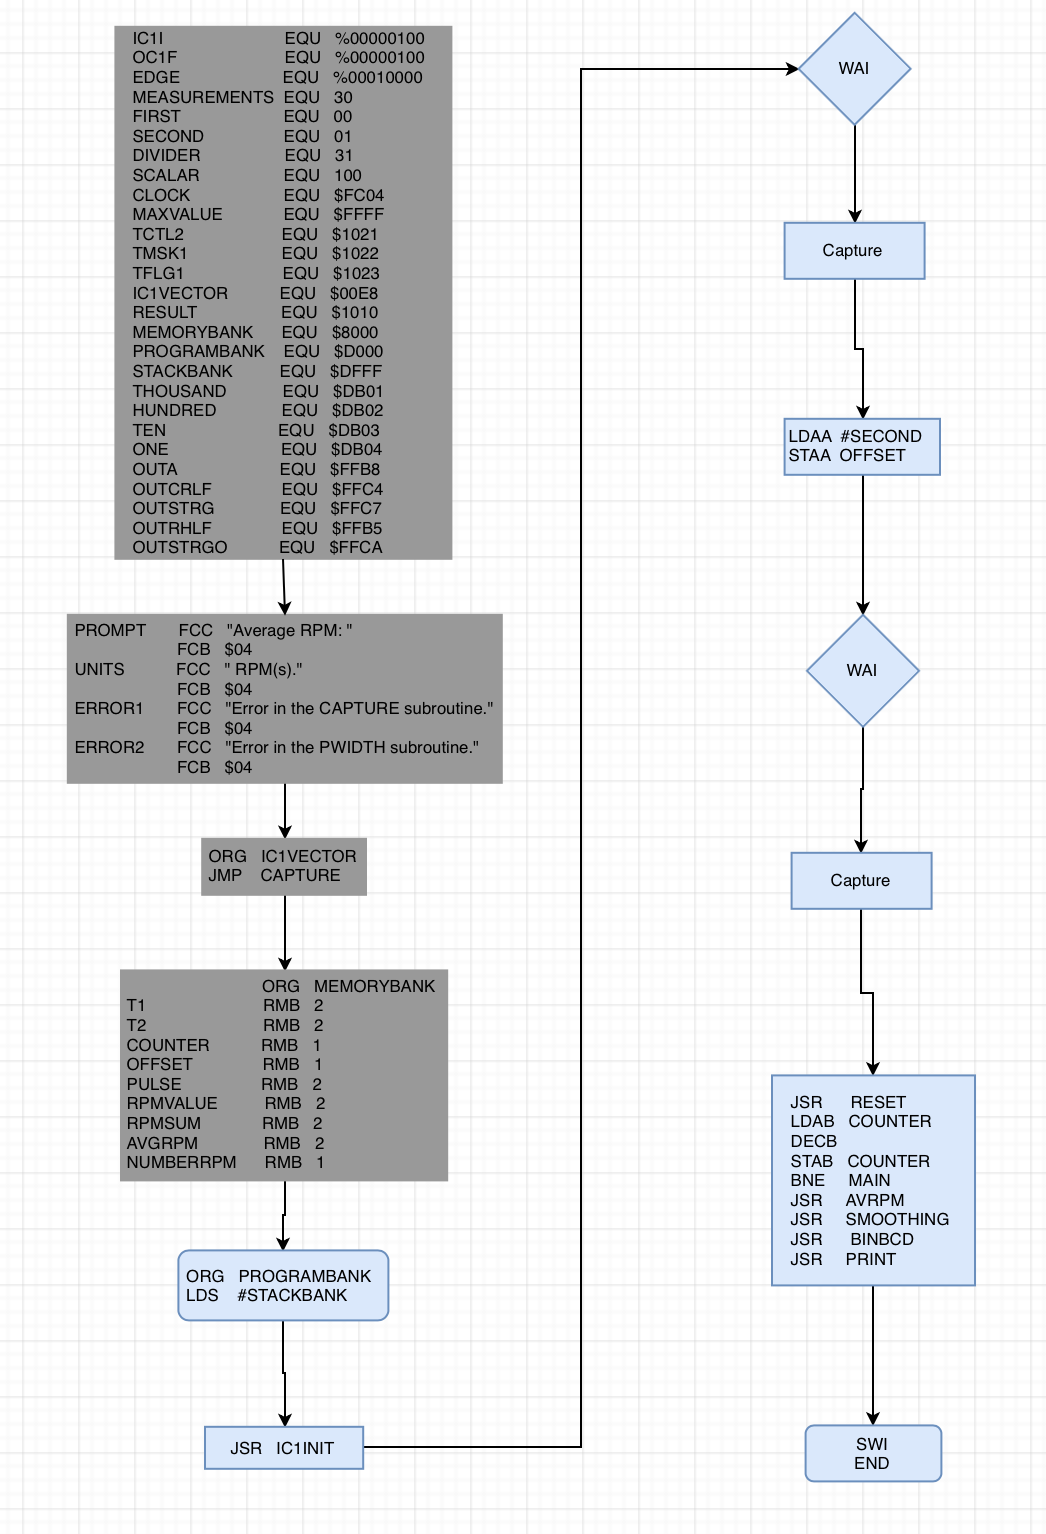
\includegraphics[scale=0.83]{main.PNG}
     \newpage{}
     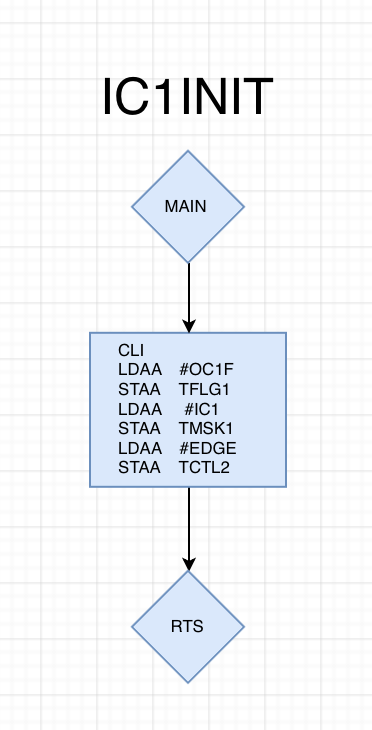
\includegraphics[scale=0.73]{init.PNG}\\
     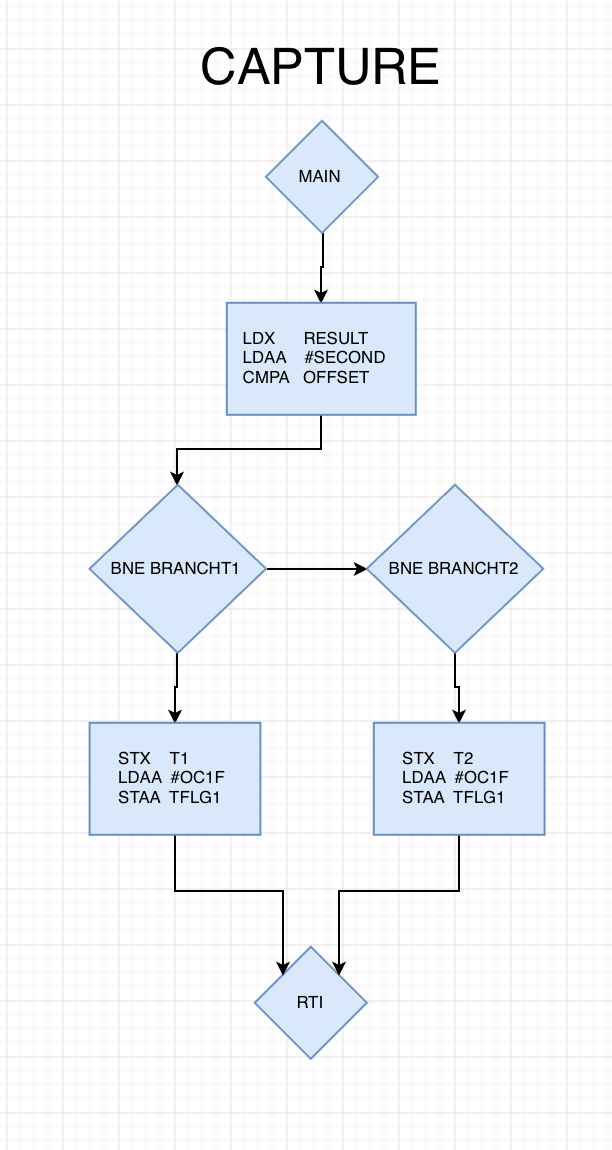
\includegraphics[scale=0.66]{cap.PNG}
     \newpage{}
     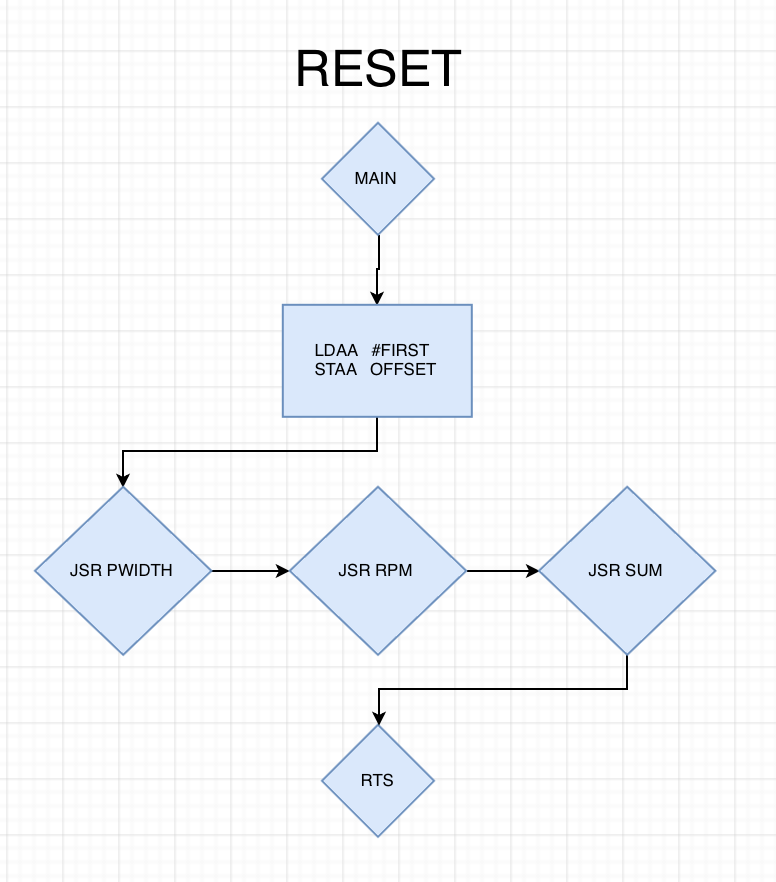
\includegraphics[scale=0.66]{reset.PNG}\\
     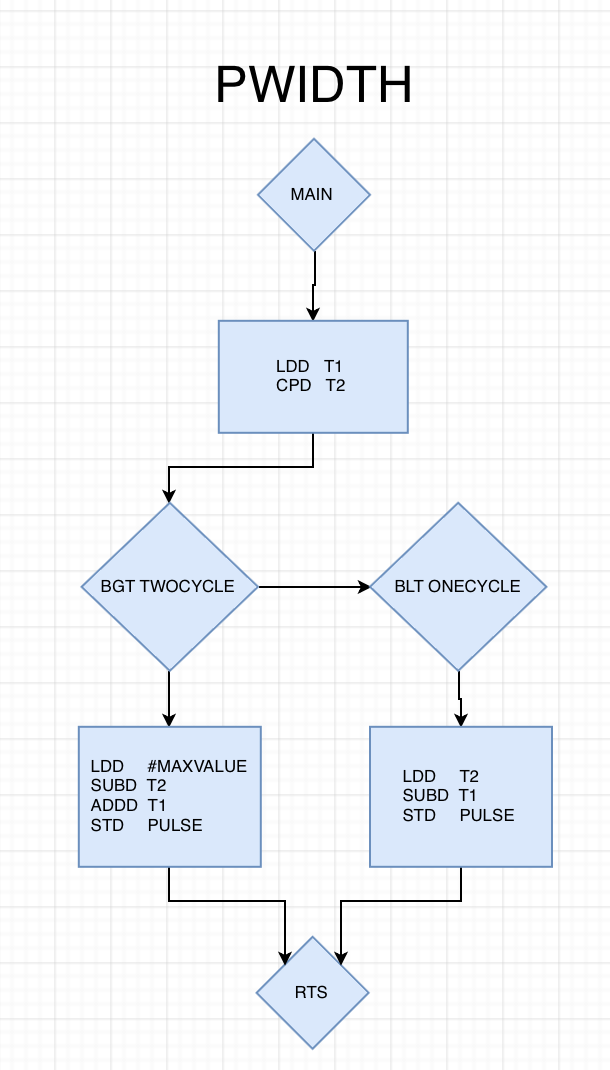
\includegraphics[scale=0.66]{pwidth.PNG}
     \newpage{}
     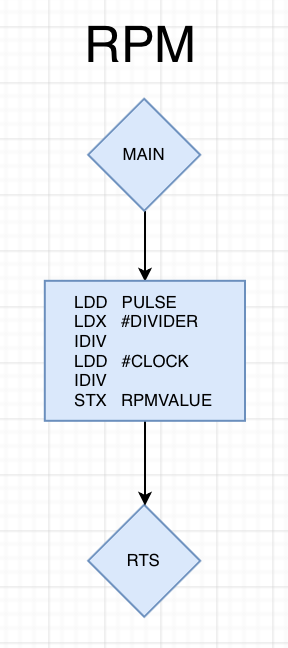
\includegraphics[scale=0.66]{rpm.PNG}
     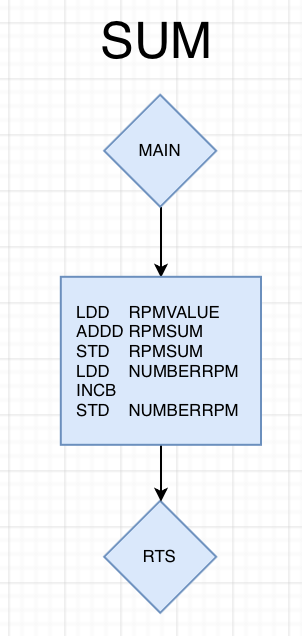
\includegraphics[scale=0.66]{sum.PNG}
     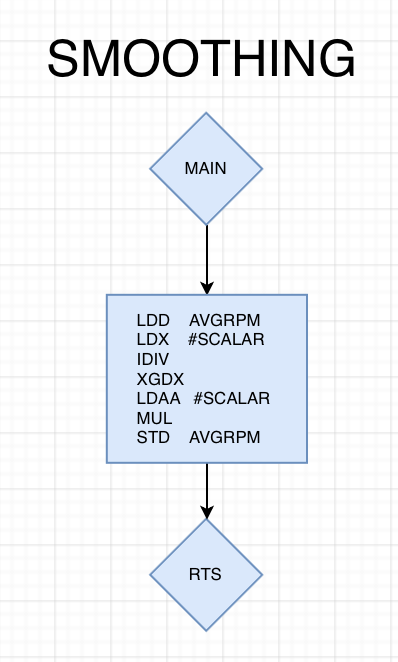
\includegraphics[scale=0.66]{smoothing.PNG}\\
     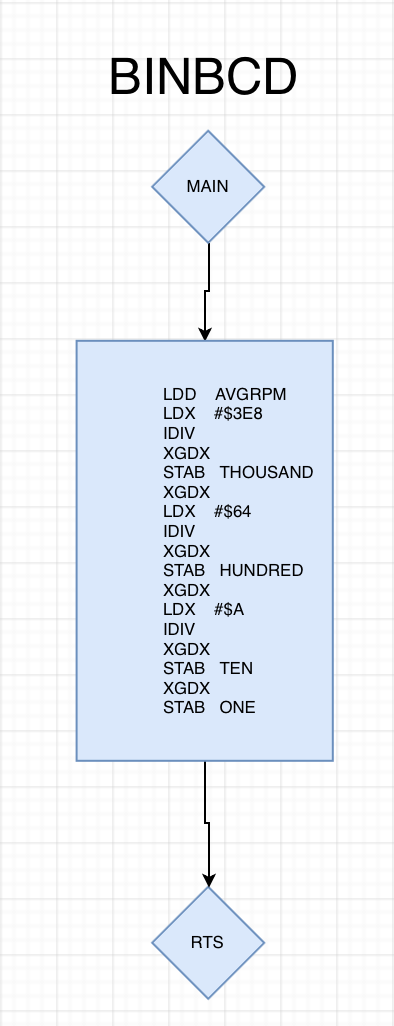
\includegraphics[scale=0.66]{bin.PNG}
     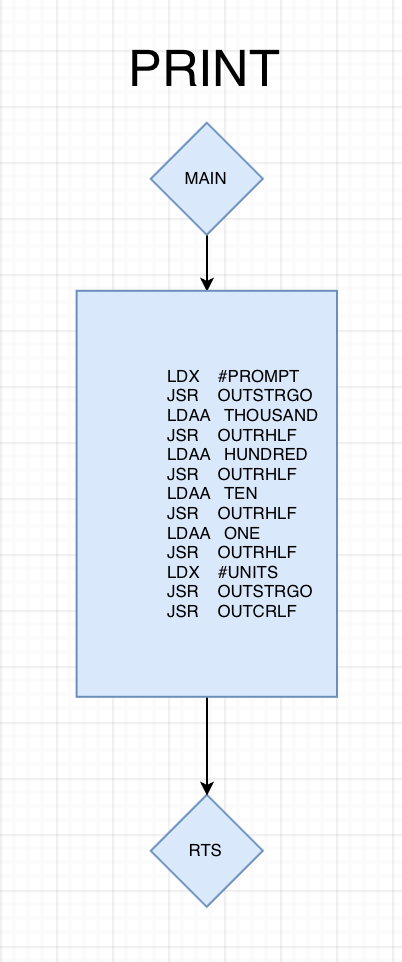
\includegraphics[scale=0.66]{print.PNG}
     \newpage{}
	\end{center}

\section*{Appendix D: Program Listing}
	\begin{Verbatim}[frame=single, fontsize=\footnotesize]
****************************************************************************************
;This bank of code is used to define all the constants that will be used in the
;following program. It defines the address of all the registers need for input
;capture as well as all the values those address will be set to. Some other
;important constants are defined to avoid the use of random numbers in the
;program and the BUFFALO provided subroutines have also had there address defined
;as well.
IC1I            EQU   %00000100 ;Set the constant IC1I to 4.
OC1F            EQU   %00000100 ;Set the constant OC1F to 4.
EDGE            EQU   %00010000 ;Set the constant EDGE to 16.
MEASUREMENTS    EQU   30        ;Set the constant MEASUREMENTS to 30.
FIRST           EQU   00        ;Set the constant FIRST to 00.
SECOND          EQU   01        ;Set the constant SECOND to 01.
DIVIDER         EQU   31        ;Set the constant DIVIDER to 31.
SCALAR          EQU   100       ;Set the constant DIVIDER to 100.
CLOCK           EQU   $FC04     ;Set the constant CLOCK to 64,516.
MAXVALUE        EQU   $FFFF     ;Set the constant MAXVALUE to 65,535.
TCTL2           EQU   $1021     ;This is the address of the T Control.
TMSK1           EQU   $1022     ;This is the address of the T Mask.
TFLG1           EQU   $1023     ;This is the address of the T Flag.
IC1VECTOR       EQU   $00E8     ;This is the address of the IC1 sudo-vector.
RESULT          EQU   $1010     ;This is the address of the TIC at interrupt.
MEMORYBANK      EQU   $8000     ;Set the starting address of the program variables.
PROGRAMBANK     EQU   $D000     ;Set the starting address of the program itself.
STACKBANK       EQU   $DFFF     ;Set the starting address of the stack pointer.
THOUSAND        EQU   $DB01     ;The memory address of the thousands digit.
HUNDRED         EQU   $DB02     ;The memory address of the hundreds digit.
TEN             EQU   $DB03     ;The memory address of the tens digit.
ONE             EQU   $DB04     ;The memory address of the ones digit.
OUTA            EQU   $FFB8     ;This subroutine outputs a character.
OUTCRLF         EQU   $FFC4     ;This subroutine outputs a carriage return.
OUTSTRG         EQU   $FFC7     ;This subroutine outputs index register X.
OUTRHLF         EQU   $FFB5     ;This outputs the right nibble of a memory byte.
OUTSTRGO        EQU   $FFCA     ;This outputs index register X without a return.
****************************************************************************************

****************************************************************************************
;These messages are using in the output of the program to make the results more
;readable to the user.  It names what the result is and its units.
PROMPT          FCC   "Average RPM: "
                FCB   $04
                
UNITS           FCC   " RPM(s)."
                FCB   $04
                
;There are two subroutines in this program that end with a couple of branching
;statements.  If for some reason the code does not branch correctly these
;messages are printed and there is a software interrupt to help with debugging.
ERROR1          FCC   "Error in the CAPTURE subroutine."
                FCB   $04
                
ERROR2          FCC   "Error in the PWIDTH subroutine."
                FCB   $04
****************************************************************************************

****************************************************************************************
;This is the address of the sudo-vector that corresponds to Input Capture 1
;interrupts.  When an interrupt occurs we want the program to begin running the
;CAPTURE subroutine.
                ORG   IC1VECTOR ;Set the origin address to the value of IC1VECTOR.
                JMP   CAPTURE   ;Jump to the CAPTURE subroutine.
****************************************************************************************

****************************************************************************************
;These are all of the variables that will be needed to run this program and all
;are stored starting at memory address $8000.
                ORG   MEMORYBANK ;Set the address origin to $8000.
T1              RMB   2          ;This is the value of TIC on the first rising edge.
T2              RMB   2          ;This is the value of TIC on the second rising edge.
COUNTER         RMB   1          ;This is a counter that tracks 30 RPM measurements.
OFFSET          RMB   1          ;This offset determines whether to use T1 or T2.
PULSE           RMB   2          ;This is the difference between T1 and T2.
RPMVALUE        RMB   2          ;The is the pulse converted into RPMs.
RPMSUM          RMB   2          ;This is a sum of all the measured RPMs.
AVGRPM          RMB   2          ;This is the average of all the RPM measurements.
NUMBERRPM       RMB   1          ;This is a counter of the number of RPM measures.
****************************************************************************************

                ORG   PROGRAMBANK ;This is the starting address of our program.
                LDS   #STACKBANK  ;This is the starting address of our stack pointer.

;We wanted to take 30 RPM measurements in our program. This limits our max RPM
;to be measured to 2100 RPMs (2100*30 = 63000), but the motors max is 2000 RPMs
;so it wont be an issue. We also wanted to initialize RPMSUM, NUMBERRPM, and
;OFFSET at the beginning of the program to insure there is no random garbage
;stored there at the start.
                LDAA  #MEASUREMENTS ;Load ACC A with 30.
                STAA  COUNTER       ;Store ACC A into the variable counter.
                LDD   #0000         ;Load ACC D with 0.
                STD   RPMSUM        ;Store ACC D into RPMSUM.
                STD   NUMBERRPM     ;Store ACC D into NUMBERRPM.
                STAA  OFFSET        ;Store ACC A into OFFSET.

;This is the MAIN of our program.  Here we initialize our Input Capture 1 by
;calling the IC1INIT subroutine and wait twice for the two rising edges. In
;between the two waits we change the value of offset which toggles whether the
;TIC is stored in T1 or T2.  After returning from the second interrupt we call
;the reset subroutine and decrement our counter. Finally we will loop back
;through the MAIN 30 total times.  After completing the 30th measurement we
;average the RPM measuremts, smooth/calibrate the value, change it to binary
;coded decimal, and print it out the terminal.
                JSR   IC1INIT   ;Jump to IC1INIT subroutine.
MAIN:           WAI             ;Waiting for an interrupt.
                LDAA  #SECOND   ;Load ACC A with 1.
                STAA  OFFSET    ;Store ACC A into the OFFSET variable.
                WAI             ;Waiting for an interrupt.
                JSR   RESET     ;Jump to the RESET subroutine.
                LDAB  COUNTER   ;Load ACC B with COUNTER.
                DECB            ;Decrement the value of COUNTER.
                STAB  COUNTER   ;Store the decremented value back into COUNTER.
                BNE   MAIN      ;If the counter is not 0, loop back to MAIN.
                JSR   AVRPM     ;Jump to the AVRPM subroutine.
                JSR   SMOOTHING ;Jump to the SMOOTHING subroutine.
                JSR   BINBCD    ;Jump to the BINBCD subroutine.
                JSR   PRINT     ;Jump to the PRINT subroutine.
                SWI             ;Software interrupt.
                END             ;The end of out program.

****************************************************************************************
;This subroutine is only run once in our program at the beginning and its
;purpose is to initialize Input Capture 1 to be prepared for an interrupt. We set
;the T Flag and T Mask to 4 or making the third bit from the right to 1 to use
;Input Capture 1.  We then set the T Control to 16 or the EDGE1 A and B to 01.
;That means that Input Capture 1 is going to wait on a Rising Edge.
IC1INIT:        CLI             ;Clearing the interrupt mask.
                LDAA  #OC1F     ;Load ACC A with the value in OC1F (4).
                STAA  TFLG1     ;Store that value in T Flag.
                LDAA  #IC1I     ;Load ACC A with the value in IC1I (4).
                STAA  TMSK1     ;Store that value in T Mask.
                LDAA  #EDGE     ;Load ACC A with the value in EDGE (16).
                STAA  TCTL2     ;Store that value in T Control.
                RTS             ;Return from the subroutine.
****************************************************************************************

****************************************************************************************
;This subroutine is what is called when the program is interrupted in the MAIN.
;That means this subroutine is called every time a rising edge occurs during
;wait. The subroutine then loads the TIC at that rising edge, checks OFFSET to
;see if this value is intended for T1 or T2, and branches to the correlated
;subroutine.
CAPTURE:        LDX   RESULT   ;Load IND X with the value of the TIC at interrupt.
                BNE   BRANCHT1 ;If the compare yields non-zero, branch to T1.
                BEQ   BRANCHT2 ;If the compare yields zero, branch to T2.
                LDX   #ERROR1  ;If both fail (unlikely) and error message is loaded.
                JSR   OUTSTRG  ;Prints the error message to the terminal.
                SWI            ;Software Interrupt.

;If this is the first interrupt this subroutine is called by capture. It stores
;the value of the TIC at the time of the interrupt into T1 and clears the T Flag
;by setting the corresponding bit to 1 and returns back to the MAIN from the
;interrupt.
BRANCHT1:       STX   T1    ;Store the value of IND X into T1.
                LDAA  #OC1F ;Loads ACC A with the value in OC1F (4).
                STAA  TFLG1 ;Stores the value of ACC A into the T Flag.
                RTI         ;Returns from the interrupt.

;If this is the second interrupt this subroutine is called by capture. It stores
;the value of the TIC at the time of the interrupt into T2 and clears the T Flag
;by setting the corresponding bit to 1 and returns back to the MAIN from the
;interrupt.
BRANCHT2:       STX   T2    ;Store the value of IND X into T2.
                LDAA  #OC1F ;Loads ACC A with the value in OC1F (4).
                STAA  TFLG1 ;Stores the value of ACC A into the T Flag.
                RTI         ;Returns from the interrupt.
****************************************************************************************

****************************************************************************************
;This subroutine is called by the MAIN when the first and second interrupts have
;already occured. It resets the OFFSET value back to 0 so the next RPM measurement
;will start over at T1. It then jumps to calculate PWIDTH, RPM, and SUM.
RESET:          LDAA  #FIRST ;Loads ACC A with 0.
                STAA  OFFSET ;Stores ACC A into OFFSET.
                JSR   PWIDTH ;Jumps to the PWIDTH subroutine.
                JSR   RPM    ;Jumps to the RPM subroutine.
                JSR   SUM    ;Jumps to the SUM subroutine.
                RTS          ;Return from the subroutine.
****************************************************************************************

****************************************************************************************
;This subroutine is called by RESET and that means that it is called everytime
;both T1 and T2 are measured.  It determines whether T1 or T2 are larger and
;branches to one of two equations based on that state.
PWIDTH          LDD   T1       ;Loads ACC D with the value in T1.
                CPD   T2       ;Compares T1 and T2 with subtraction.
                BGT   TWOCYCLE ;If the compare is more than zero, it calls TWOCYCLE.
                BLT   ONECYCLE ;If the compare is less than zero, it calls ONECYCLE.
                LDX   #ERROR2  ;If both fail (unlikely) and error message is loaded.
                JSR   OUTSTRG  ;Prints the error message to the terminal.
                SWI            ;Software Interrupt.
                
;This subroutine is called by PWIDTH to calculate the value of the PULSE when T1
;and T2 are both captured within one cycle. In other words this is used if the
;TIC does not wrap around between T1 and T2 captures. It then subtracts T1 from
;T2 and stores that in pulse.
ONECYCLE:       LDD   T2    ;Loads ACC D with the value in T2.
                SUBD  T1    ;Subtracts T1 from the value in ACC D.
                STD   PULSE ;Stores the value in ACC D into PULSE.
                RTS         ;Return from the subroutine.

;This subroutine is called by PWIDTH to calculate the value of the PULSE when T1
;and T2 are captured within two cycles. In other words this is used if the
;TIC does wrap around between T1 and T2 captures. It then subtracts T1 from
;2-byte max and adds T2 and stores that in pulse. It is essentially the
;difference between T1 and T2 while subtracting away the wrap of $FFFF.
TWOCYCLE:       LDD   #MAXVALUE ;Loads ACC D with 65,535.
                SUBD  T1        ;Subtracts the value in T1 from ACC D.
                ADDD  T2        ;Adds the value in T2 to ACC D.
                STD   PULSE     ;Stores the value in ACC D into PULSE.
                RTS             ;Return from the subroutine.
****************************************************************************************

****************************************************************************************
;This subroutine is called by the RESET function which means that it is called
;every time that T1 and T2 have been captured. The previous subroutine used those
;measurements to calculate the value of PULSE, or the number of clock cycles
;between T1 and T2. It then uses a ratio equal to 2 Million/PULSE to calculate
;the RPMVALUE.  This is done because 2 Million will not fit into a 2-byte number.
;We divide both the numerator and the denominator by 31 giving us 64,516/PULSE.
;Because 2 Million and PULSE will not evenly divide by 31 this is where we will
;lose our accuracy.
RPM:            LDD   PULSE    ;Load ACC D with the value of PULSE.
                LDX   #DIVIDER ;Load IND X with the value 31.
                IDIV           ;Divide ACC D by IND X.
                LDD   #CLOCK   ;Load ACC D with 64,516.
                IDIV           ;Divide ACC D by IND X.
                STX   RPMVALUE ;Store IND X (Result) into RPMVALUE.
                RTS            ;Return from the subroutine.
****************************************************************************************

****************************************************************************************
;This subroutine is called by RESET which means that it is called every time T1
;and T2 have been captured.  Its PULSE and RPMVALUE have already been calculated
;which means all that is left to do is add the measurement to the running sum to
;later be divided by the number of measurements for an average.
SUM:            LDD   RPMVALUE  ;Load ACC D with the value of RPMVALUE.
                ADDD  RPMSUM    ;Add RPMSUM to the value of ACC D.
                STD   RPMSUM    ;Store ACC D back into RPMSUM.
                LDD   NUMBERRPM ;Load ACC D with the value of NUMBERRPM.
                INCB            ;Increment ACC B by 1.
                STD   NUMBERRPM ;Store the value of ACC D back into NUMBERRPM.
                RTS             ;Return from the subroutine.
****************************************************************************************

****************************************************************************************
;This subroutine is called by the MAIN and is only called once all 30, or number
;equal to COUNTER, measurements have been taken because we only want to calculate
;the average RPM once we have all the measurements. The subroutine divides the
;running RPMSUM by the NUMBERRPM counter and stores that value in AVGRPM. Again
;it is likely that we will lose some accuracy to truncation here.
AVRPM:          LDD   RPMSUM    ;Load ACC D with the value of RPMSUM.
                LDX   NUMBERRPM ;Load IND X with the value of NUMBERRPM.
                IDIV            ;Divide ACC D by IND X.
                STX   AVGRPM    ;Store IND X (Result) into AVGRRPM.
                RTS             ;Return from the subroutine.
****************************************************************************************

****************************************************************************************
;This subroutine is called after all the measurements have been captured and the
;average RPM has been calculted.  As mentioned earlier all of the divisions are
;likely to cause a lose of accuracy and this smoothing subroutine essentially
;truncates the 2 least significant digits as they are not accurate, due to these
;divisions. We attempted to do a calibration formula but due to the size of
;AVGRPM and limitations of assembly it only made the measurements less accurate.
;This is an imperfect solution to the problem. If you intend on measuring a
;frequency using non-zero 10s and 1s digits the JSR to this subroutine should be
;commented out and even still the returned values will be imperfect.
SMOOTHING:      LDD    AVGRPM   ;Load ACC D with the value of AVGRPM.
                LDX    #SCALAR  ;Load IND X with the value of DIVIDER.
                IDIV            ;Divide ACC D with IND X.
                XGDX            ;Swap IND X with ACC D.
                LDAA   #SCALAR  ;Load ACC A with the value of DIVIDER.
                MUL             ;Multiply the value of A with B
                STD    AVGRPM   ;Store ACC D (Result) into AVGRPM.
                RTS             ;Return from the subroutine.
****************************************************************************************

****************************************************************************************
;This subroutine is called once all the calculations are done by the MAIN and it
;is used to code the AVGRPM in hexidecimal into decimal so that it can later be
;printed out the terminal in decimal for the user.
BINBCD:         LDD    AVGRPM   ;Load ACC D with the value of AVGRPM.
                LDX    #$3E8    ;Load IND X with the value of 1000.
                IDIV            ;Divide ACC D by IND X.
                XGDX            ;Swap IND X with ACC D.
                STAB   THOUSAND ;Store the right nibble of ACC D into address $DB01.
                XGDX            ;Swap IND X with ACC D.
                LDX    #$64     ;Load IND X with the value of 100.
                IDIV            ;Divide ACC D by IND X.
                XGDX            ;Swap IND X with ACC D.
                STAB   HUNDRED  ;Store the right nibble of ACC D into address $DB02.
                XGDX            ;Swap IND X with ACC D.
                LDX    #$A      ;Load IND X with the value of 10.
                IDIV            ;Divide ACC D by IND X.
                XGDX            ;Swap IND X with ACC D.
                STAB   TEN      ;Store the right nibble of ACC D into address $DB03.
                XGDX            ;Swap IND X with ACC D.
                STAB   ONE      ;Store the right nibble of ACC D into address $DB04.
                RTS             ;Return from the subroutine.
****************************************************************************************

****************************************************************************************
;This subroutine is called by the main after everything has been calculated and
;the AVGRPM has been converted to binary coded decimal. The subroutine echos the
;right nibble of each of the four address from the BINBCD subroutine to the
;terminal, which represents each of the four digits in base 10 of AVGRPM.
PRINT:          LDX    #PROMPT  ;Load IND X with the message at PROMPT.
                JSR    OUTSTRGO ;Jump to the OUTSTRGO subroutine to echo IND X.
                LDAA   THOUSAND ;Load ACC A with the value at $DB01.
                JSR    OUTRHLF  ;Jump to the OUTRHLF subroutine to echo ACC A LB.
                LDAA   HUNDRED  ;Load ACC A with the value at $DB01.
                JSR    OUTRHLF  ;Jump to the OUTRHLF subroutine to echo ACC A LB.
                LDAA   TEN      ;Load ACC A with the value at $DB01.
                JSR    OUTRHLF  ;Jump to the OUTRHLF subroutine to echo ACC A LB.
                LDAA   ONE      ;Load ACC A with the value at $DB01.
                JSR    OUTRHLF  ;Jump to the OUTRHLF subroutine to echo ACC A LB.
                LDX    #UNITS   ;Load IND X with the message at UNITS.
                JSR    OUTSTRGO ;Jump to the OUTSTRGO subroutine to echo IND X.
                JSR    OUTCRLF  ;Jumps to the OUTCRTL subroutine to echo a return.
                RTS             ;Return from the subroutine.
****************************************************************************************
   \end{Verbatim}
	
\section*{Appendix E: Temperature Measurements}
	\begin{center}
		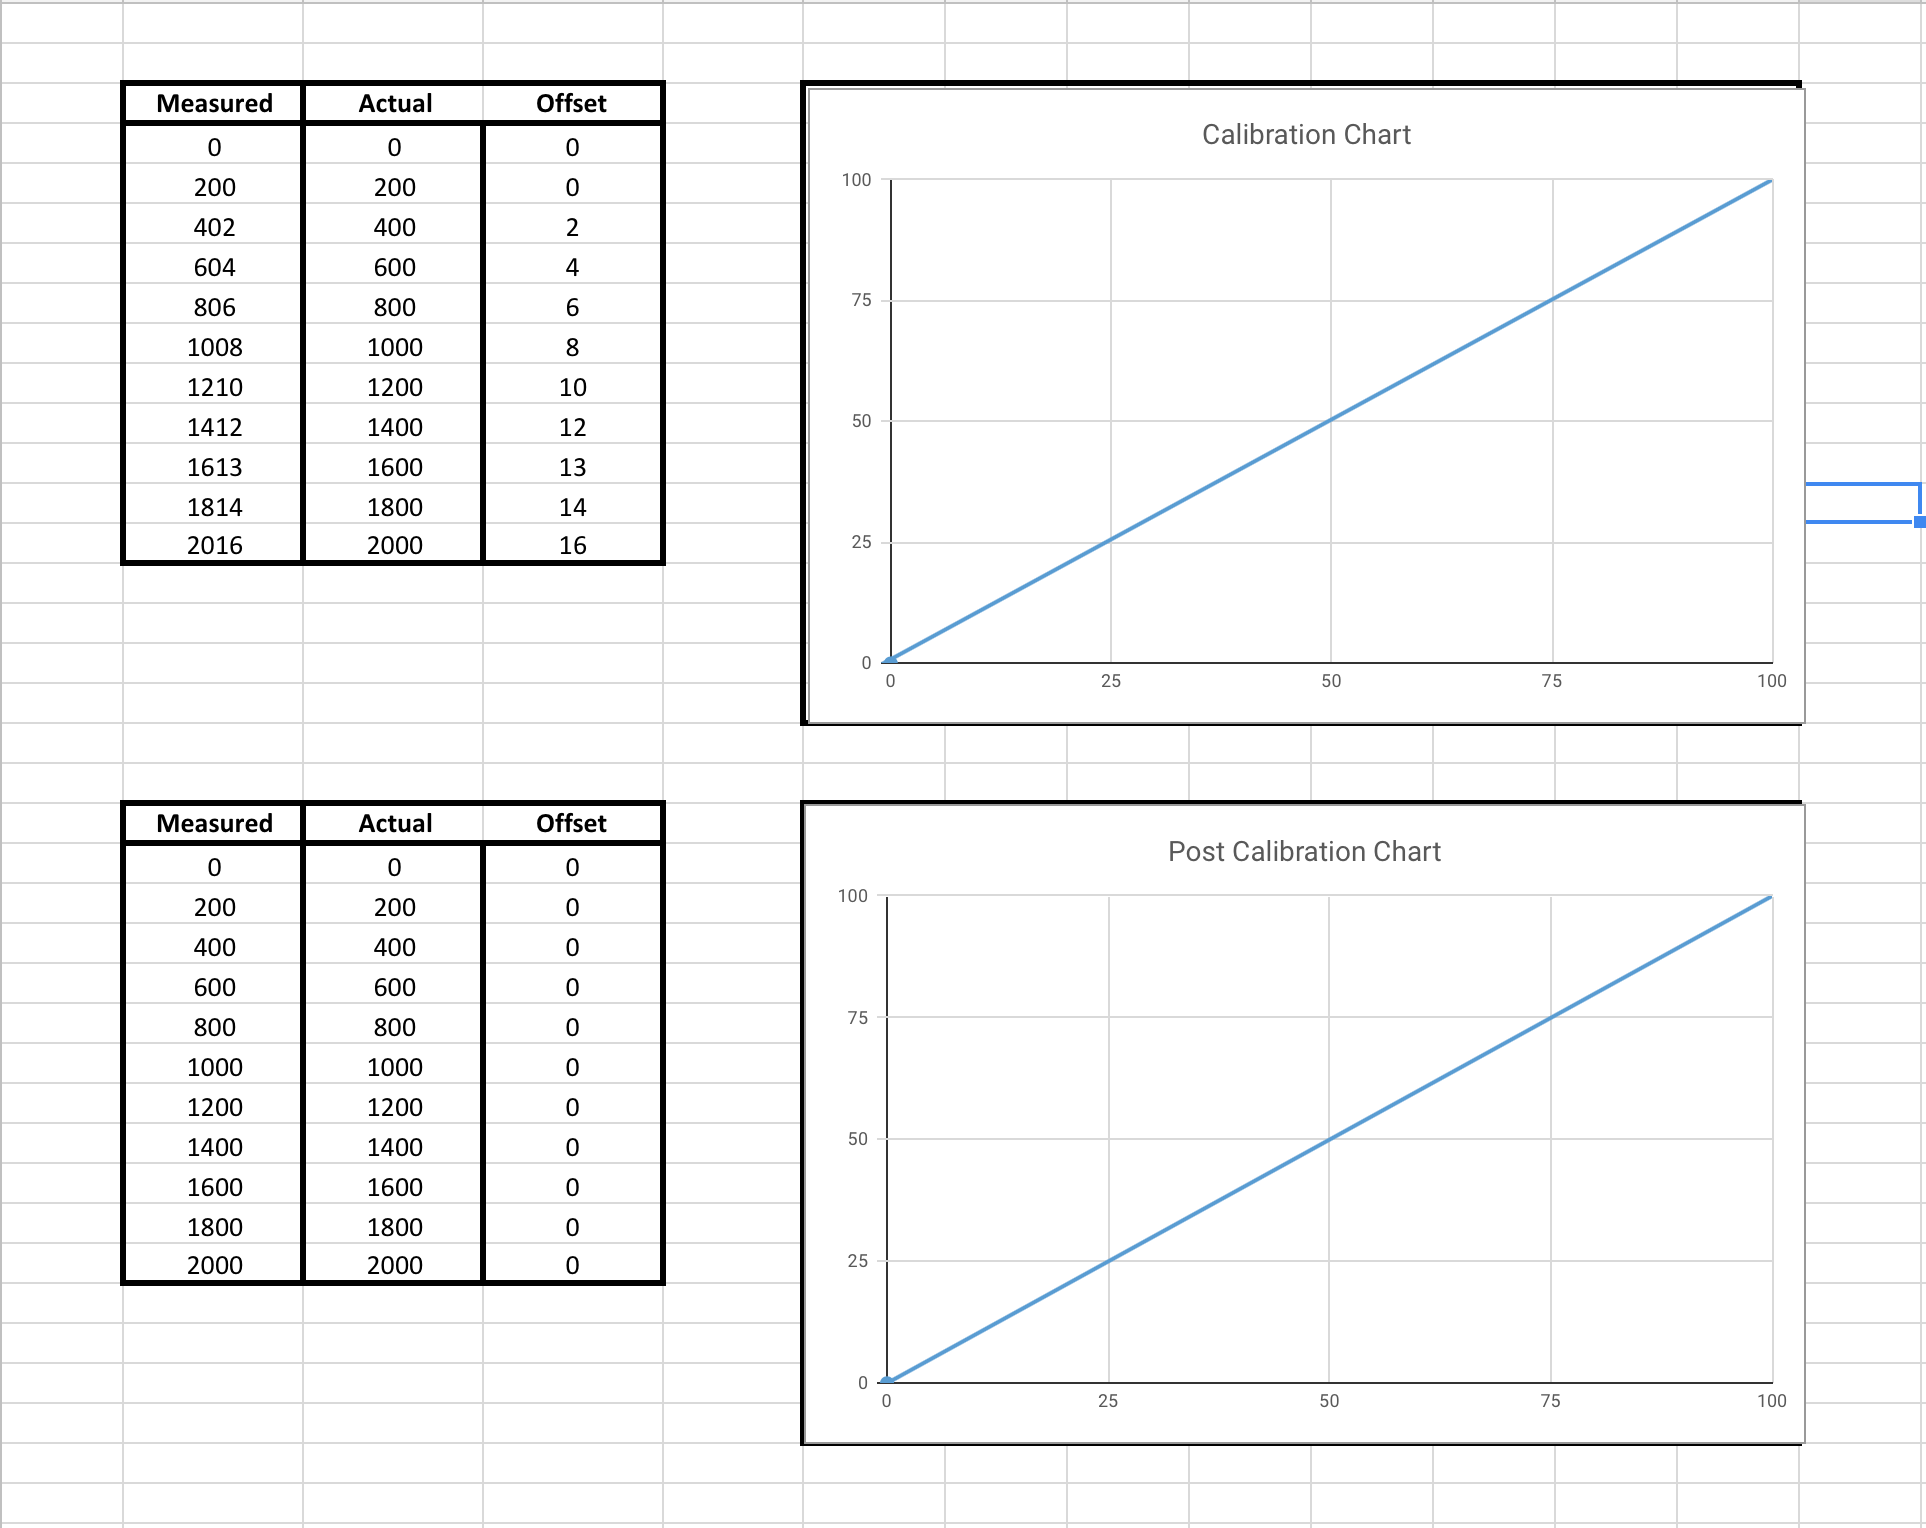
\includegraphics[scale=.48]{chart.PNG}
		Calibration Equartion $Y = 0.9880x + 0.1801$
	\end{center}
\end{document}